\chapter{植物の育成要素}
(これをどこの章に入れるべきか)
\begin{figure}[b] 
    \centering
    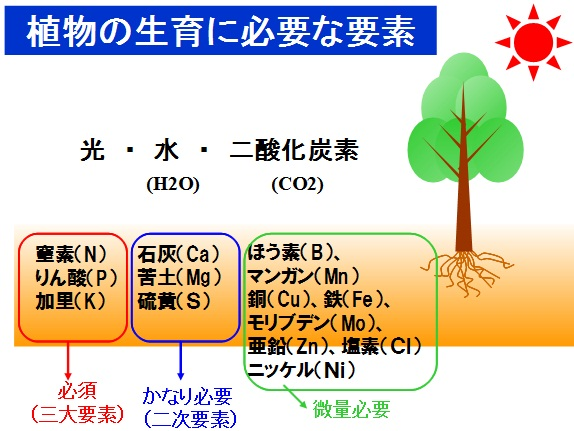
\includegraphics[width=0.7\textwidth]{image/plants/283856.jpg}
    \caption{植物の育成に必要な要素}
    \label{plants_youso}
\end{figure}
植物の育成に必要な要素としてFig.\ref{plants_youso}示すように光、水、空気の3つがひつようになる。
更に、健全な育成を行う為には温度、栄養の2つを適切に管理する必要がある。
つまり、植物が自律的に育成するにはこれら5つの要素をモニタする必要がある。
\par しかし、通常空間において空気中の酸素や二酸化炭素の量は高度が変化しない限り、その濃度に変化は少ない。
特に限定された空間内において、ロボットを使った実験を行うような場合は、空気の変化は少ないと思われる。
また、空気中の変化を観測し適切でない場合においても、それは限定された空間内全てにおいて同じことが当てはまる。
つまり、空気をモニタする必要はないとする。
\par 次に、土壌の栄養素に関してはその観測が難しく、植物の生育に必要となるものは10種を超え、ロボットが自身で測定することは現実的ではない。
そこで土壌の栄養を鉢植え時に調整し、育成に十分は量を投与する。
土壌栄養素のモニターは無視し、土壌の栄養は常に最適な状態で固定されることとなる。
\par よって、比較的容易な3つの要素をモニタ対象とする。
\section{光}
植物は動物と異なり、日の出ている日中は光合成を行い、日のない時は動物のように呼吸を行う。
育成に必要な光は日光、電球、蛍光灯、LEDの放つ光で成長が確認されている。
近年の研究では、赤色と青色の光を放つLEDの光が植物の育成に最も効果的と報告されている。
しかし、蛍光灯でも育成には十分な効果が得られ、本実験では広く一般的な照明器具である蛍光灯の光を用いて植物を育成を行う。
\par そこで、本研究では光合成に必要となる光を照度と捉え、必要照度をモニタする。
\section{水}
生物は水なしでは生命維持が困難である。
これは植物も同様で、光合成の過程で水分が必要となる。
水分は外部より供給を行い、一度土壌に蓄えられた後に植物に水分が行き渡るよ。
\par そこで、本研究では土壌に蓄えられた水分量を植物自身の水分量と捉え、これモニタする。
\section{温度}
温度も同様に適切な状態でないと育成を妨げる。
植物の種類により適切な温度は異なり、他2つの要素より実験環境に大きく左右されることになる。
\par そこで、実験環境内で育成が可能な植物の種類の選択を行い、外気温度のモニタを行う。

